\documentclass[12pt,letterpaper]{article}

\usepackage[bookmarks=true]{hyperref}
\usepackage{graphicx}
\usepackage{geometry}
\usepackage{fontspec}
\usepackage{xunicode}
\usepackage{xltxtra}
\usepackage{color,colortbl}
\usepackage{url}
\usepackage[table]{xcolor}
\usepackage{multirow}
\usepackage{xtab}
\usepackage[final]{pdfpages}
\usepackage{subfigure}
\usepackage{amsmath,amssymb}


\definecolor{Gray}{gray}{0.9}

\defaultfontfeatures{Mapping=tex-text} % converts LaTeX specials (``quotes'' --- dashes etc.) to unicode

\setromanfont [Ligatures={Common}]{Cardo}
\setmonofont{Inconsolata}

% Set your name here
\def\name{Patrick J. Martin}

% Replace this with a link to your CV if you like, or set it empty
% (as in \def\footerlink{}) to remove the link in the footer:
\def\footerlink{}

% The following metadata will show up in the PDF properties
\definecolor{darkblue}{rgb}{0.0,0.0,0.5}
\hypersetup{
  colorlinks = true,
  linkcolor=darkblue,
  urlcolor = darkblue,
  pdfauthor = {\name},
  pdftitle = {\name: PJM Application},
  pdfpagemode = UseNone
}

\geometry{
  body={6.5in, 8.5in},
  left=1.0in,
  top=1.0in,
  bottom=1.0in
}

\subfigcapmargin = .5cm

% Customize page headers
\pagestyle{myheadings}
\markright{\name}
\thispagestyle{empty}

% Custom section fonts
\usepackage{sectsty}
\sectionfont{\rmfamily\mdseries\Large}
\subsectionfont{\rmfamily\mdseries\large}

% Don't indent paragraphs.
\setlength\parindent{0em}

% Make lists without bullets
\renewenvironment{itemize}{
  \begin{list}{}{
    \setlength{\leftmargin}{1.5em}
  }
}{
  \end{list}
}

% courtesy D. Hovemeyer
\newenvironment{denseItemize}{%
\begin{list}{}{\setlength{\itemsep}{0.4em}\setlength{\leftmargin}{1.5em}\setlength{\parsep}{0in}}}{\end{list}}
%\setlength{\topsep}{.1mm}

\begin{document}

\pagestyle{myheadings}
\markright{\name---Project 1: Boston Housing Prices}
\thispagestyle{empty}

%{\LARGE \name} \\
%\smallskip
%\smallskip
{\Large Project 1: Boston Housing Prices} \\ 
Patrick Martin \\
\rule{\columnwidth}{1pt}

\vspace{1em}

This project required synthesis of introductory modeling and evaluation material.
Using the provided code skeleton, I modified four sections of the code to collect basic statistics from provided data, implement a performance metric, analyze the learning curves and model complexity, and tune a \texttt{DecisionTreeRegressor} algorithm.

\section*{Statistical Analysis of Housing Data}

The Boston housing data contained {\bf 506} entries that each have {\bf 13} features. Using \texttt{numpy} array functions, I determined the following statistical measures:
\begin{itemize}
	\item Minimum home price = {\bf 5.0}
	\item Maximum home price = {\bf 50.0}
	\item Mean home price = {\bf 22.5328}
	\item Median home price = {\bf 21.2}
	\item Standard deviation = {\bf 9.188}
\end{itemize}

\section*{Model Evaluation}

Home prices are based on continuous numerical values (or, drawn from $\mathbb{R}$).
Consequently, predicting a new home price based on current home price data is a {\bf regression} problem.
Choosing an error-based metric fits the problem, since we want the prediction algorithm to place values as close as possible to comparable homes.
In particular, I selected the {\bf mean-squared error} metric to penalize incorrect predictions far more than an absolute error.
The other scoring mechanisms discussed in class (e.g. precision, recall) make most sense for classification problems, not regression. \\

When you tune a machine learning algorithm, you have to keep in mind the tradeoff between error and complexity.
If you overfit the algorithm, it will be too sensitive to outlier data; however, if you underfit the algorithm, it will have poor prediction performance.
The tuning of the \texttt{DecisionTreeRegressor} used a 70/30 split of the provided housing data set using the simple function call to \verb|train_test_split|.
By pulling out 70\% of the data randomly for training data, it will lessen the chance of bias, or under-fitting, into the predictor.
Overall, we need to provide as much un-biased training data to the learning algorithm so that we get a better learning result.
\\

The cross validation tool we used in this project was \verb|GridSeachCV| that accepts a candidate algorithm, the parameters of interest, and a scoring function.
By leveraging a known algorithm, the best \verb|max_depth| of the \verb|DecisionTreeRegressor| is computed with an exhaustive search.
My particular implementation uses the same \verb|mean_squared_error| performance metric and passes in the \verb|max_depth| parameter array.
Performing an exhaustive cross validation operation prevents the algorithm from being tuned to a particular subset of the housing data set.
Otherwise, the algorithm could possibly favor cluster of data to make an incorrect prediction.
If \verb|train_test_split| were the only method used to tune the algorithm, we would likely introduce more variance sensitivity in the model.
The default \verb|GridSeachCV| performs a 3-fold cross-validation process that diversifies the training data.
Doing so allows for this particular data to be used three more times to train the model.

\section*{Model Performance}

\begin{figure}[h!]
	\centering
	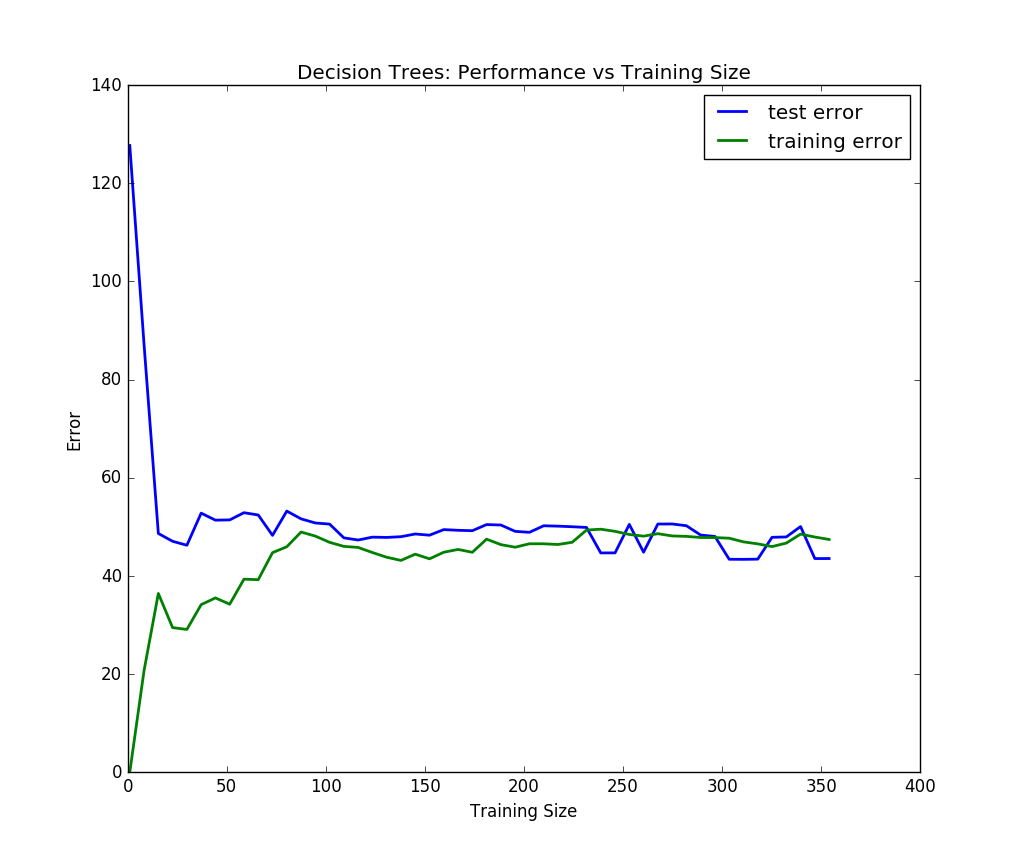
\includegraphics[width=0.65\textwidth]{dt-learningcurve-1.png}
	\caption{A plot of the training and test data error over size of training. This image is the initial run with the decision tree \texttt{depth = 1}.}
	\label{fig:lc1}
\end{figure}

The provided skeleton code created a loop to increase the maximum decision tree depth size and plot the error results. 
Figures \ref{fig:lc1} and \ref{fig:lc10} illustrate these curves for different \verb|max_depth| values.
By examining these figures (and the ones generated at run time) the {\bf training error approaches a plateau} as the depth of the decision tree increases and as the amount training data is increased.
With a lower depth, like Figure \ref{fig:lc1}, this plateau results in a very large training error, but the error hovers around the test data error.
The {\bf testing error decreases} as the size of the training data set increases.
{\bf Although the testing and training error decrease, there still remains an gap between the results}, even at a high \verb|max_depth| value. \\

\begin{figure}[h!]
	\centering
	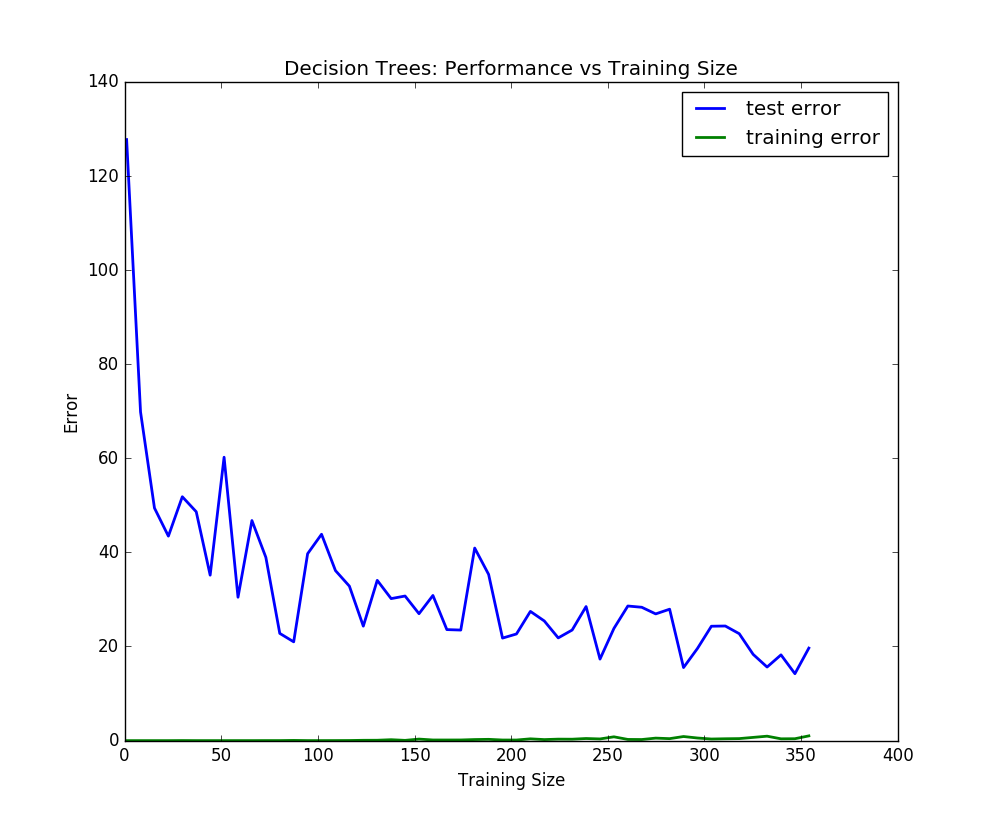
\includegraphics[width=0.65\textwidth]{dt-learningcurve-10.png}
	\caption{This image shows the error with a decision tree \texttt{depth = 10}.}
	\label{fig:lc10}
\end{figure}

Figure \ref{fig:lc1} shows an interesting case where there is {\bf considerable bias} with \verb|max_depth=1|.
When the depth increases to 10, the training error drops significantly as the training data size increases.
The test error also drops, but does not converge to the training error curve.
These plots indicate that the algorithm is fully trained with at least 200 data points.
This model still has variance, due to the difference between training data error and test data error.
Figure \ref{fig:lc10} demonstrates that the model still suffers from {\bf high variance} since the the test and training test error remain separated by about 20.
One interesting trend is that the plots based on depths 5 through 10 do not increase the test error significantly.
This observation indicates that higher depth does not always mean better performance for the added computational cost. \\


By plotting the test error against the depth of the the \verb|DecisionTreeRegressor|, shown in Figure \ref{fig:mc}, I get confirmation of the trend seen in the learning curves.
Although {\bf training error approaches 0}, the test error continues to {\bf remain between 10 and 20}.
Given this plot, I would recommend a \verb|DecisionTreeRegressor| model with \verb|max_depth| $\in \{4,5,6\}$.

\begin{figure}[h!]
	\centering
	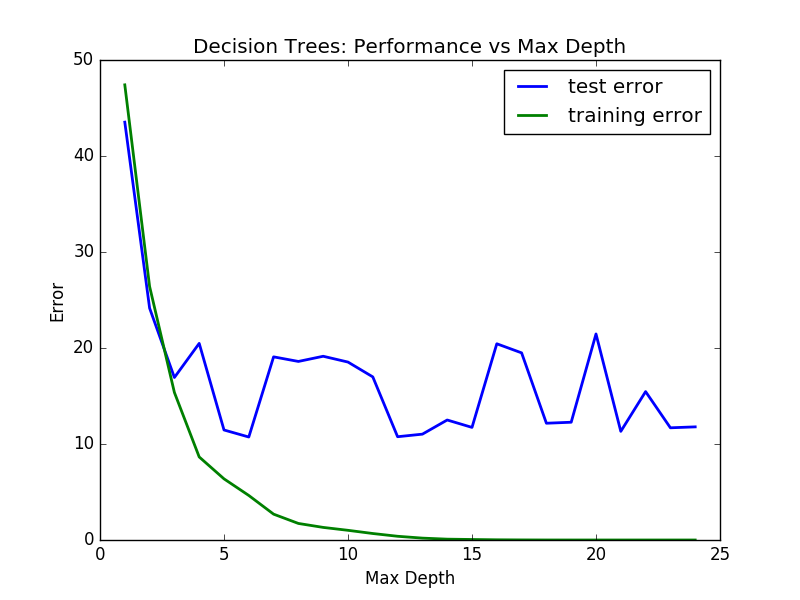
\includegraphics[width=0.65\textwidth]{model-complexity.png}
	\caption{A graph of the model complexity as the depth of the decision tree increases.}
	\label{fig:mc}
\end{figure}

\section*{Model Prediction}

Using the \verb|GridSearchCV| discussed before, I ran the program several times.
On the whole, the tuned model resulting from this grid search based on mean-squared error had a \verb|max_depth=4|, with the occasional value of \verb|5| or \verb|6|.
One sample run of the main program iterated the model fit function five times and I saw the following output:
\begin{center}
	\verb|depth = [4, 6, 9, 4, 4]|
	\verb|predictions = [21.6297, 20.7659, 19.3272, 21.6297, 21.6297]|
\end{center}
These results confirm that the grid search tunes to model to favor a {\bf tree depth of 4}. \\

The predictions from this tuned estimator appear to be near the mean and median home prices. In fact, they are easily within one standard deviation of the mean.
The course so far has not discussed much about the output of these algorithms, other than that they are ``predictors'' based on prior data. 
How would we actually know at this point whether this prediction are reasonable other than seeing the {\bf learning curves reducing} and that the {\bf predicted value is near the mean}?




\end{document}